These records retain their original classifications and limitations. Moving them changes presentation, not their outcomes or evidentiary status.

\subsection*{Historical Fixed-Scale Image-Space Diagnostics}
\label{subsec:tradeoff}

Table~\ref{tab:sweep} reproduces the 13-scale sweep reported in the submitted 01549 manuscript. We retain it to preserve the original development question, but the object-level outputs, full run manifest, and metric implementation mapping are not available in the current authority. Its values and Figures~\ref{fig:curve}--\ref{fig:heatmap} are therefore historical diagnostics, not a new reanalysis or confirmatory evidence.

\begin{table}[t]
\centering
\caption{Historical 01549 report of a 13-scale sweep on the stated 50-object set. Values are reproduced from the submission and have not been independently recomputed from row-level outputs; they are retained as development diagnostics.}
\label{tab:sweep}
\small
\begin{tabular}{lcccc}
\toprule
Scale & $\Delta$FG-SSIM$\uparrow$ & POS & $\Delta$Crop-SSIM$\uparrow$ & $\Delta$PSNR$\uparrow$ \\
\midrule
0.75 & $-$0.013 & 20/50 & +0.113 & 7.53 \\
0.90 & +0.024 & 30/50 & +0.137 & 8.32 \\
1.00 & +0.047 & 34/50 & +0.147 & 8.79 \\
1.10 & +0.070 & 36/50 & +0.159 & 9.08 \\
1.15 & +0.071 & 36/50 & +0.157 & 9.25 \\
1.25 & +0.088 & 37/50 & +0.161 & 9.37 \\
1.35 & +0.100 & 39/50 & +0.163 & 9.63 \\
1.50 & +0.113 & 40/50 & +0.163 & 9.76 \\
1.60 & +0.120 & 42/50 & +0.166 & 9.83 \\
1.75 & +0.127 & 43/50 & +0.173 & 9.97 \\
2.00 & +0.134 & 44/50 & +0.169 & 9.96 \\
2.25 & +0.142 & 43/50 & +0.175 & 9.91 \\
2.50 & +0.145 & 44/50 & +0.165 & 9.91 \\
\bottomrule
\end{tabular}
\end{table}

The submitted table reports a rising $\Delta$FG-SSIM over most of the listed scale range and a near-plateau in the crop metric at higher settings. We retain this reported pattern only as historical motivation: absent row-level outputs and a complete run manifest, we do not treat it as an independently confirmed scale-response law. It motivates asking whether a single aggregate structural score fully describes the effect of adapter scaling.

\begin{figure}[t]
\centering
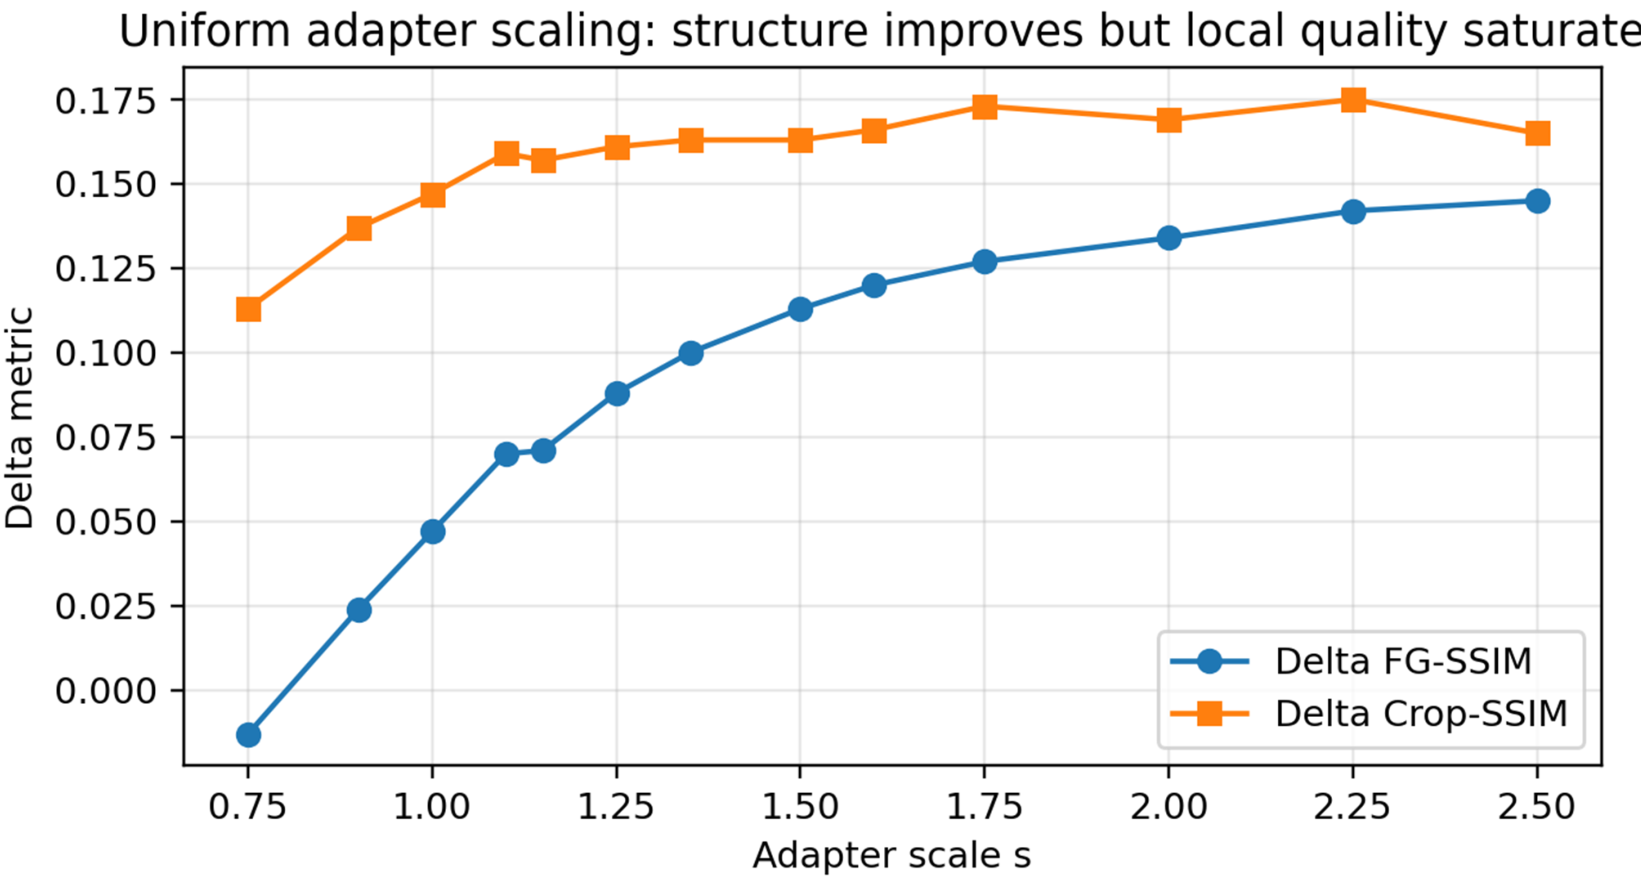
\includegraphics[width=\columnwidth]{fig2.pdf}
\caption{Historical fixed-scale diagnostic from the submitted 01549 paper. The plotted source reports FG-SSIM and Crop-SSIM over adapter scales; the underlying object-level run records are not available for independent reanalysis. It motivates measuring more than one endpoint, but is not a current confirmatory result.}
\label{fig:curve}
\end{figure}

The submitted heatmap depicts object-level variation across the reported scales, but its underlying rows cannot be reconstructed from the current evidence archive. We retain the visual diagnostic as part of the 01549 research history and do not infer a population-level response distribution from it. The updated Fresh C analysis below uses its own frozen cohort and matched inputs.

\begin{figure}[t]
\centering
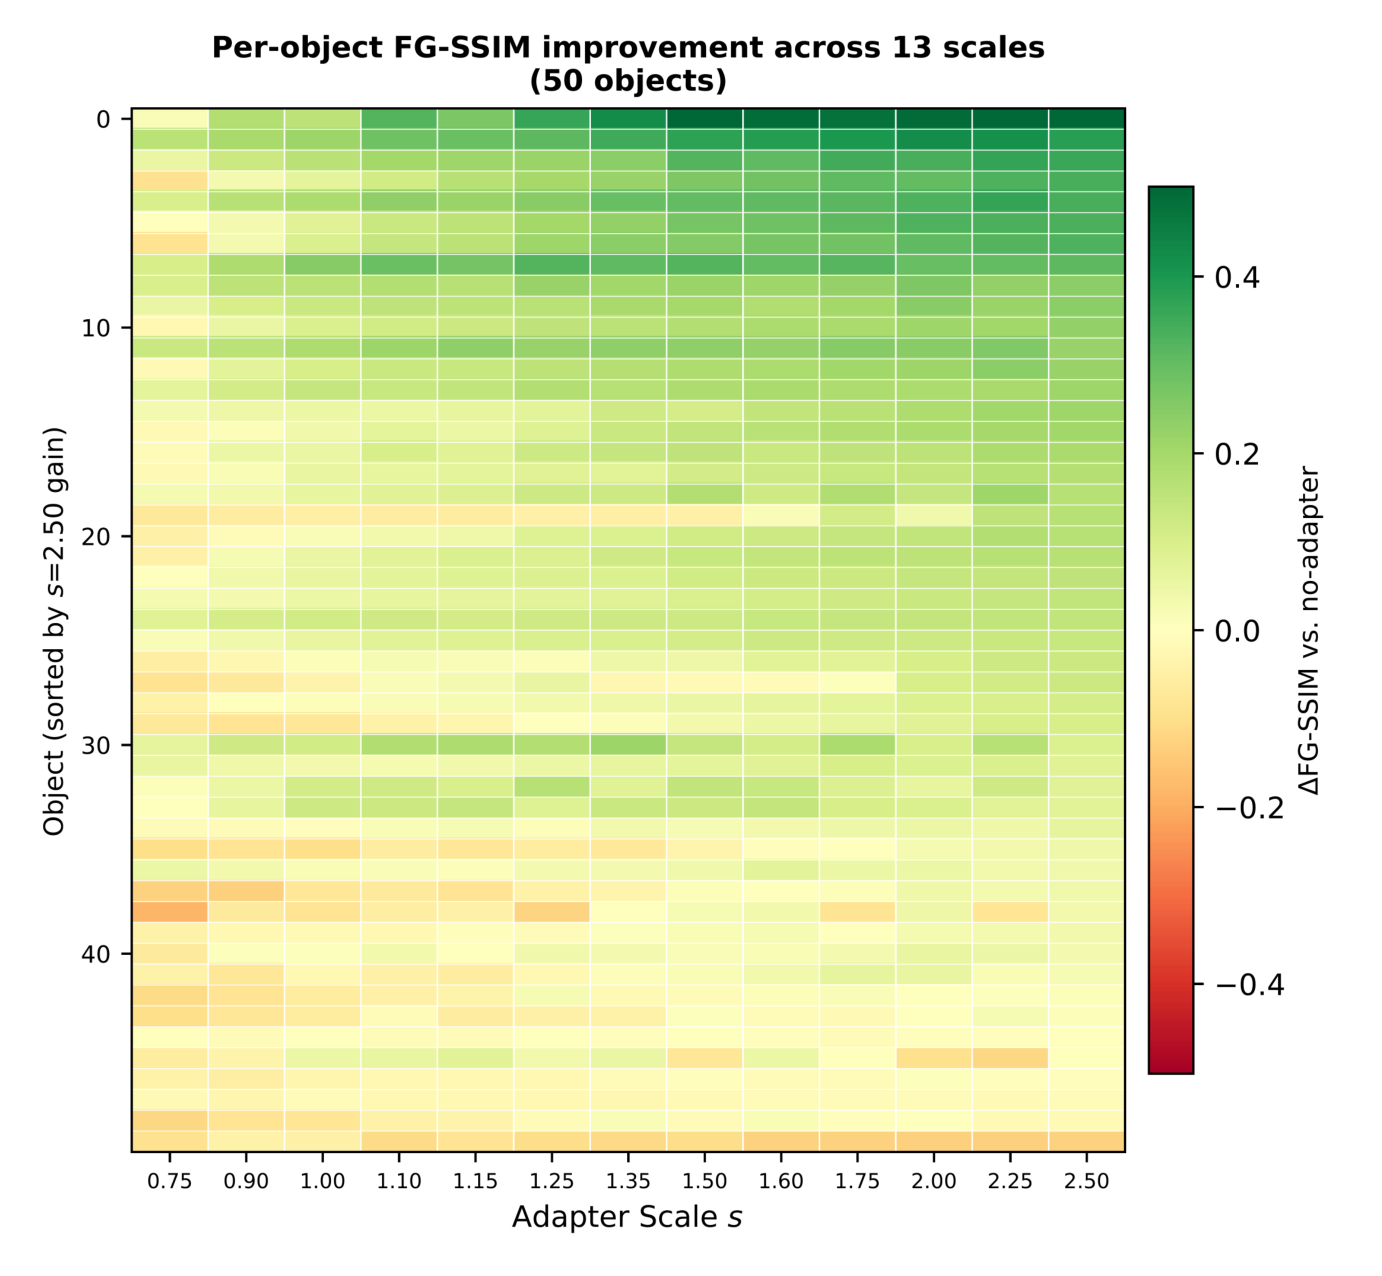
\includegraphics[width=\columnwidth]{fig3.pdf}
\caption{Historical per-object $\Delta$FG-SSIM heatmap reproduced from the 01549 submission (50 objects, 13 scales). The plot illustrates the originally reported response variation; row-level provenance is incomplete, so it is not used for a current population inference.}
\label{fig:heatmap}
\end{figure}

\subsection*{C3 Development Record and Current Evaluation}
\label{subsec:c3}

The submitted paper records 17 uniform, layer-wise, and timestep-conditioned variants on a 24-object development probe and identifies C3 as its chosen profile. This study question remains relevant: does a stage-dependent request offer a useful control setting beyond a single global scale? Because the complete historical row-level data and selection provenance are not available in the current authority, the original Table~\ref{tab:probe} and Figure~\ref{fig:pareto} are retained as historical development records, not as a verified ranking or proof of optimality. Fresh C evaluates the recorded C3 profile without another schedule search.

\begin{table}[t]
\centering
\caption{Representative values reported for the historical 24-object, 17-variant development probe. The full candidate set is shown in Figure~\ref{fig:pareto}. The underlying row-level outputs and selection-time provenance are not available for independent reanalysis; the table records the submitted development result and does not establish an optimum.}
\label{tab:probe}
\footnotesize\setlength{\tabcolsep}{3pt}
\begin{tabular}{llcc}
\toprule
Variant & Reported category & $\Delta$FG-SSIM & $\Delta$Lap Var \\
\midrule
C4 & Late-stage high & 0.105 & $-$0.0120 \\
C2 & Timestep schedule & 0.104 & $-$0.0110 \\
B2 & Layer-wise schedule & 0.090 & $-$0.0135 \\
A\_s2.00 & Uniform & 0.087 & $-$0.0062 \\
C3 & Mid-stage high & 0.084 & $-$0.0006 \\
A\_s2.25 & Uniform & 0.079 & $-$0.0096 \\
A\_s2.50 & Uniform & 0.078 & $-$0.0108 \\
B6 & Layer-wise schedule & 0.000 & $-$0.0027 \\
\bottomrule
\end{tabular}
\end{table}

The original table and plot use shape and texture-variation proxies to describe the development choice. They do not establish that texture was faithful to the reference, nor that C3 was the unique best candidate. In this revision, C3 is therefore described as the historical profile carried forward for matched evaluation, not as a theorem-derived or globally optimal schedule.

The requested profile is piecewise constant over normalized sampling progress $p$:
\begin{equation}
s_{\mathrm{req}}(p) =
\begin{cases}
1.25, & 0 \le p < 1/3,\\
2.50, & 1/3 \le p < 2/3,\\
1.25, & 2/3 \le p \le 1,
\end{cases}
\qquad \mathrm{C3}=(1.25,2.50,1.25).
\end{equation}
This is an inference-time instruction on the existing adapter path; no weights are trained. Its tested value is task- and implementation-specific. The schedule operation itself is not claimed as a new general primitive.

\begin{figure*}[!t]
\centering
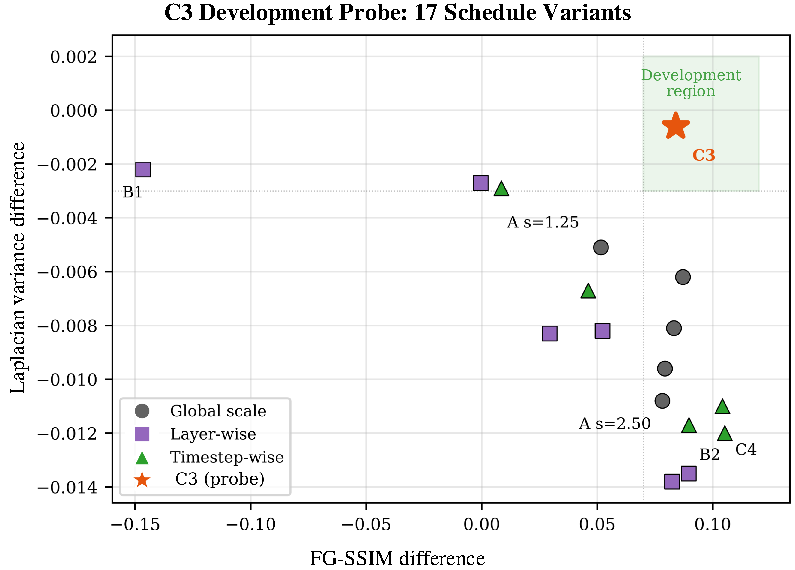
\includegraphics[width=0.78\textwidth]{figures/fig7_c3_development.pdf}
\caption{Historical 17-variant development probe from the submitted 01549 paper (24 objects). The axes show changes in FG-SSIM and Laplacian variance; variance is a texture-variation diagnostic, not a fidelity measure. “C3” identifies the selected historical profile, not an optimum or general schedule law. The candidate-level outputs are unavailable for independent reanalysis.}
\label{fig:pareto}
\end{figure*}

The source Figure~5 (26-object texture ratios) is not included as an active result because its object IDs, selection trace, and metric lineage are incomplete. The original 24-object Table~3 is moved to Supplementary Section S10 as a verbatim historical diagnostic, with no texture-fidelity or population inference. Both source assets remain preserved in the authenticated submission and forensic archive; neither decision removes the fixed-scale research question or the development record of C3.


\subsection*{Applied-Scale Budget and Temporal Placement}
\label{subsec:temporal-placement}

Fresh C compares the recorded C3 profile with GFL under the same frozen checkpoint, runner, seed policy, inputs, and target views. Its applied deep/middle scale sums are 82.5 for C3 and 62.5 for GFL, while the shallow sum is 40 for both after the 0.8 cap. The registered C3--GFL improvement therefore combines a change in middle-third strength with a larger per-group nominal budget; it does not isolate temporal placement.

A separate post-inspection placement analysis used the clean-v2 strict-276 cohort and a common runner within that run. It is not the Fresh C cohort, and it is not an independent replication of the historical 24-object selection probe. Temporal L--L--H means low requests during early and middle steps and high requests during late steps; it uses a different shallow-group control from Fresh C's layer-conditioned LLH addendum. The latter requests (1.25,1.25,2.50) in deep/middle and (0.50,0.50,0.75) in shallow; the older global placement comparison keeps shallow capped at 0.8. Neither is identical to the new 16-step Late-high condition. With 50 steps, the strict-276 run assigns 17/16/17 steps to the three windows. C3 and temporal L--L--H have near-matched applied-scale sums (82.50 versus 83.75 in deep and middle; 40 in shallow), but their post-scale residual magnitudes are not matched.

\begin{table*}[t]
\centering
\scriptsize
\setlength{\tabcolsep}{4pt}
\caption{Post-inspection strict-276 placement analysis. Entries are C3 minus temporal L--L--H with pointwise 95\% object-bootstrap intervals; positive PSNR/SSIM and negative LPIPS differences favor C3. Temporal L--L--H is favored on all six formal endpoints. The analysis is separate from Fresh C, and its scalar sums do not match realized residual dose.}
\label{tab:temporal-placement}
\begin{tabular}{lcc}
\toprule
Endpoint & Mean difference [95\% CI] & Direction \\
\midrule
Full-view PSNR (dB) & $-0.268100$ [$-0.311101,-0.227797$] & L--L--H \\
FG-PSNR (dB) & $-0.177084$ [$-0.230539,-0.130784$] & L--L--H \\
FG-SSIM & $-0.008851$ [$-0.011455,-0.006291$] & L--L--H \\
Edge-SSIM & $-0.035301$ [$-0.036581,-0.034031$] & L--L--H \\
FG-LPIPS & $+0.001896$ [$+0.001205,+0.002578$] & L--L--H \\
Full-view LPIPS & $+0.008658$ [$+0.007465,+0.009831$] & L--L--H \\
\bottomrule
\end{tabular}
\end{table*}

Against the fixed-mean profile, C3's strict-276 FG-PSNR difference is $+0.502875$~dB (95\% CI $[+0.462018,+0.542244]$). These results show sensitivity to the tested stage allocation, not a universally preferred placement or an equal-realized-dose effect.

Fresh B is a separate $N=150$ cohort and reports LLH against LFM-EXACT, not C3. The paired LLH--LFM-EXACT differences are $+0.325$~dB FG-PSNR (95\% CI $[+0.209,+0.446]$) and $-0.00460$ FG-LPIPS (95\% CI $[-0.00563,-0.00357]$); both intervals fall within the recorded practical margins of $\pm0.5$~dB and $\pm0.01$. The saved lock states a pre-run freeze time, but the earliest preserved commit containing it is later than that time. We therefore report Fresh B as retrospective sensitivity rather than authenticated preregistered confirmation.

A separate Core-7 summary uses the same 276 object labels and recorded checkpoint lineage as Fresh C but does not establish common runner or complete input-tensor identity across its seven conditions. Its post-hoc C3--GFH contrasts point in opposite directions for Full-view PSNR ($+0.725229$~dB, 95\% CI $[+0.647134,+0.806467]$) and FG-PSNR ($-1.214235$~dB, 95\% CI $[-1.313952,-1.114705]$). It remains a retrospective diagnostic, not a same-runner confirmation or reproduction of the original $+0.96$~dB result (Supplementary Section~S5).


\subsection*{Layer-by-Window Sensitivity}
\label{subsec:layerwindow}

The A2 and A3b maps test response heterogeneity over three adapter groups and five denoising windows. Their object-cluster statistics describe variation within the tested interventions; they are not effect estimates for a dose-independent schedule mechanism.

\begin{table}[t]
\centering
\scriptsize
\setlength{\tabcolsep}{3pt}
\caption{Object-cluster tests of the observed layer-by-window response maps. A2 is exploratory; A3b is retrospective Fresh B sensitivity because the preserved history cannot authenticate pre-run availability of its lock. Interaction share and cell RMSE summarize the observed map, not a causal effect.}
\label{tab:layerwindow-main}
\begin{tabular}{llrrr}
\toprule
Map, cohort & Endpoint & Wald $W(8)$ & Reported $p$ & Share; cell RMSE \\
\midrule
A2, $N=300$ & FG-PSNR & 1879.963 & $<10^{-300}$ & 56.8\%; 0.1222~dB \\
A2, $N=300$ & FG-LPIPS & 481.081 & $8.04\times10^{-99}$ & 43.5\%; 0.001695 \\
A3b, $N=150$ & FG-PSNR & 525.700 & $3.43\times10^{-107}$ & 36.0\%; 0.0205~dB \\
A3b, $N=150$ & FG-LPIPS & 225.015 & $5.37\times10^{-43}$ & 14.0\%; 0.000342 \\
\bottomrule
\end{tabular}
\end{table}

The earlier A3b common-support calculation compared 10-step integrated raw $L_2$ norms across three layer groups. The saved corrections have different spatial resolutions (24$\times$16, 48$\times$32, and 96$\times$64), and the traces omit channel counts, so absolute norms are dimension-dependent across groups. We withdraw the reported 0/2,250 overlap as a cross-layer dose-support conclusion. Together with the Fresh B lock chronology, A3b remains retrospective sensitivity evidence. Its map shows response heterogeneity under the tested interventions, but does not identify a dose-independent layer-by-window effect or an optimal schedule.

A separate retrospective analysis on the \texttt{FRESH\_CONFIRM\_300} cohort found nine of ten plus-one-corrected associations between LLH--GFL image-space deltas and ground-truth descriptors; the FG-LPIPS/coverage test had adjusted $p=0.0508$. FG-PSNR means ranged from $+4.140$~dB in the lowest Laplacian-variance quartile to $-0.087$ and $-0.029$~dB in the upper two quartiles. These are cohort-specific associations, not a causal complexity effect, a threshold, a schedule selector, or a texture-fidelity result.


\paragraph{Native deployment and training controls.}
Two-object diagnostics separately examine full-pipeline sampling, image features, classifier-free guidance, target resolution, geometry encoding and conditional/\allowbreak unconditional residual branches. None of these isolated changes fully repairs the reference-appearance failures. An audit of the recorded custom trainer identifies repeated-top supervision and conditional-only execution despite a declared conditioning-drop probability. These findings support checking the executed protocol rather than attributing the failure to one interface factor. Complete grids and all negative diagnostics are retained in Supplementary Sections S21--S25.

A new protocol uses native 512-pixel unique-six-view supervision, actual positive/negative reference conditioning and fixed 2000-update training on 1090 input-valid training objects with zero Fresh C UID overlap. Its fifty-object evaluation is frozen before this checkpoint's outputs, but the objects were previously used in research. Against geometry disabled, the HF-based geometry checkpoint improves FG-LPIPS by 0.0200 (95\% paired interval $[-0.0283,-0.0125]$, primary Holm $p<0.0001$). Equal-budget Late-high minus Fixed Mean is $+0.0027$ ($[-0.00003,+0.00640]$, adjusted $p=0.080$); it does not establish a temporal-allocation gain. None of the eighteen corrected secondary contrasts establishes C3 superiority over Fixed Mean or GFH. A full local v29 ControlNet baseline is better in PSNR, SSIM and LPIPS, but its UNet weights differ from the HF base; this is a deployment comparison rather than an isolated architecture test (S26--S28).

A same-v29-base follow-up keeps the fixed training protocol and the fifty-object cohort. Geometry improves FG-LPIPS over geometry disabled by 0.0131 ($[-0.0189,-0.0083]$; 44/50 objects improve), but remains worse than full v29 by 0.0159 ($[0.0085,0.0237]$); both primary contrasts survive Holm correction. FG-SSIM remains lower than full v29 by 0.0533 in the six-test secondary family. Nonsignificant PSNR and color differences do not establish equivalence. Matching base weights controls one confound, while geometry architectures, training histories and input representations still differ. These comparisons use the declared 50-step, seed-42, no-background-removal protocol rather than the original 75-step command-line defaults. Image endpoints combine view placement and appearance; GT foreground masking does not penalize every outside-silhouette artifact. These comparisons reuse previously observed objects and do not establish a temporal advantage or competitive quality (S29).

\paragraph{Measured deployment cost and quality.}
A two-GPU crossover benchmark compares the same-base small-geometry checkpoint with full v29 on the first five frozen objects. Each method has two warm-ups and three timed repetitions per object on each GPU (60 timed calls); every output matches the corresponding quality-matrix pixels. Table~\ref{tab:deployment-cost} reports synchronized warmed generation time and total peak allocated GPU memory, including the resident pipeline. Input disk IO, model loading, CPU geometry conversion, PNG writing and metric scoring are excluded. The per-object median latency ratios are 1.30--1.31 for full v29 divided by small geometry across the two GPUs. The denoiser-plus-geometry parameter counts are 2.57 and 3.82 billion respectively, excluding shared CLIP/VAE components; small additional geometry modules do not imply the same reduction in total model size or GPU memory. The lower measured cost is accompanied by the previously established FG-LPIPS and FG-SSIM losses against full v29. It belongs to this newly trained geometry architecture comparison, not to TCAS, and does not establish a global efficiency frontier, equal quality or an end-to-end texturing-system speedup (S30).

\begin{table}[t]\centering\scriptsize
\caption{Measured deployment cost with the known quality tradeoff. Performance uses five fixed objects and warmed repetitions; quality uses fifty previously studied objects and their five nonreference views. GPU memory is total peak allocated memory during generation, not geometry-module storage alone. Repeated calls are not independent quality samples.}
\label{tab:deployment-cost}
\begin{tabular}{llrrrr}
\toprule
GPU & Deployment & Median (s) & Peak (GiB) & FG-LPIPS & FG-SSIM \\
\midrule
0 & Full v29 & 15.71 & 14.89 & 0.0775 & 0.6937 \\
0 & Small geometry & 12.03 & 13.18 & 0.0934 & 0.6404 \\
1 & Full v29 & 14.58 & 14.89 & 0.0775 & 0.6937 \\
1 & Small geometry & 11.17 & 13.18 & 0.0934 & 0.6404 \\
\bottomrule
\end{tabular}

\end{table}


\subsection*{Cross-Interface Evaluation}
\label{subsec:cross-interface}

Table~\ref{tab:cross-interface} places the primary GeoTex path beside the auxiliary MV-Adapter and MVDiffusion interventions. The methods use different conditioning interfaces and scale semantics; object-level results are not pooled across systems.

\begin{table*}[t]
\centering
\scriptsize
\setlength{\tabcolsep}{3pt}
\caption{Interface-specific intervention evidence. Nominal budgets are described within each implementation; no cross-interface realized-dose match is available. These rows are not architecture-matched replications. The MVDiffusion contrast is reported as raw condition A minus condition B; lower FG-LPIPS, CIEDE2000, and GT-relative texture error are favorable, whereas higher PSNR, FG-SSIM, and Edge-SSIM are favorable.}
\label{tab:cross-interface}
\begin{tabular}{p{2.4cm}p{4.0cm}p{4.2cm}p{4.5cm}}
\toprule
System and injected signal & Control axis and budget & Cohort and principal result & Evidence grade and limitation \\
\midrule
GeoTex-Adapter, Fresh C &
Five-channel normal/depth/foreground adapter residuals added to UNet ResNet features; temporal requests with native layer caps. C3--GFL applied deep/middle sums differ (82.5 vs.\ 62.5); shallow sums are both 40. &
$N=300$. C3--GFL FG-PSNR is $+0.522$~dB [0.404, 0.641], but GFH and Generic Linear have more favorable means than C3 on all four displayed endpoints. &
Matched, same-runner Fresh C image-space comparison; identifies the named paired contrast, not timing alone, a schedule optimum, or baked material quality. \\
MV-Adapter, layer/window probe &
Condition guider plus decoupled multi-view attention; one of four down-block points is raised from 0.75 to 1.00 in one of five 10-step windows. Group residual-dose ratio is 1:0.57:1.46; no equal-realized-dose map was run. &
98/99 planned objects. The exploratory four-metric Holm-corrected cluster-Wald family found no interaction detected after correction (primary FG-LPIPS Holm $p=0.303$). &
Interface-specific layer/window sensitivity; not C3 temporal transfer. A corrected non-detection does not show no interaction or equivalence. \\
MV-Adapter, layer/time profile panel &
Four condition-guider features were scaled per point; L-FIX, L-LHL, and L-LLH add 228 outputs to the existing global schedules on the same 76-object Exact holdout. &
Layer-wise/global contrasts are metric-dependent. The two within-profile temporal contrasts show no consistent pattern; their 30 pointwise intervals are unadjusted. &
Retrospective: protocol and outputs first appear in one preserved commit. This feature-scaling interface differs from GeoTex residual correction and does not establish TCAS transfer. \\
MVDiffusion, compatibility interface &
Correspondence-aware decoder-side CPBlocks; the tested multiplier is a product of a layer factor and temporal scale over five blocks. The 75-object panel used the compatibility base; a later check found 1,552/1,552 loaded tensors and 12/12 views identical to the native mirror on one object. &
$N=75$, 12-view output grids, six frozen target views scored per object, and 50 steps. For raw L--LLH minus G--FL means: PSNR $-0.4538$, FG-SSIM $-0.01939$, Edge-SSIM $-0.005941$, FG-LPIPS $+0.002745$, CIEDE2000 $+1.3730$, and GT-relative texture error $-0.08229$. Full pointwise 95\% CIs for all endpoints and five contrasts are in Supplementary Table~S12. &
Within-interface, mixed endpoint comparison on a different conditioning path; the 75-object panel itself was not rerun on the mirror. No shared scale semantics, cross-system dose match, or architecture-causal inference. \\
\bottomrule
\end{tabular}
\end{table*}

Under the raw A-minus-B convention, L--LLH has higher CIEDE2000 (worse reference-color agreement) than G--FL, lower PSNR/FG-SSIM/Edge-SSIM, lower GT-relative error against the recorded variation statistics, and no separated FG-LPIPS difference. The lower variation-statistic error is not evidence of texture fidelity. The earlier negative CIEDE2000 value was an improvement-coded effect, not a raw contrast; the direction audit and all five comparisons are reported in Supplementary Table~S12.

For the 98-object MV-Adapter probe, the original additive-residual bootstrap had an invalid zero-power null and was not used for interaction inference. The exploratory object-cluster Wald test is reported with its corrected family; its non-detection does not establish absence of interaction. In the separate 76-object Exact-holdout panel, layer-wise versus global contrasts trade PSNR, color, and ground-truth-relative texture endpoints against FG- and Edge-SSIM. For temporal placement, only one of six pointwise 95\% intervals excludes zero in L-LLH versus L-FIX (direction-adjusted CIEDE2000 $+0.072790$ [$+0.004371,+0.156696$]); only one does so in G-LLH versus G-LHL (Edge-SSIM $-0.000261$ [$-0.000522,-0.000032$]). The 30 intervals are descriptive and unadjusted. The protocol and outputs first appear in the same preserved commit, so this is retrospective sensitivity evidence, not confirmation or an equivalence test. The MVDiffusion panel used a compatibility deployment; a separate check matched its loaded tensors and one object's rendered views to a native mirror, but the full panel was not rerun. These probes remain interface-specific and do not establish architecture-invariant scheduling or transfer of the GeoTex residual intervention.




